% !TeX program = xelatex
\documentclass[UTF8,11pt,a4paper,fontset=none]{ctexart}
\usepackage{fontspec}
\usepackage{xeCJK}
\IfFontExistsTF{Noto Serif CJK SC}{
  \setCJKmainfont{Noto Serif CJK SC}\setCJKsansfont{Noto Sans CJK SC}\setCJKmonofont{Noto Sans CJK SC}
}{
  \IfFontExistsTF{Droid Sans Fallback}{
    \setCJKmainfont{Droid Sans Fallback}\setCJKsansfont{Droid Sans Fallback}\setCJKmonofont{Droid Sans Fallback}
  }{
    \setCJKmainfont{Songti SC}\setCJKsansfont{PingFang SC}\setCJKmonofont{PingFang SC}
  }
}
\usepackage[a4paper,margin=2.35cm]{geometry}
\usepackage{amsmath,amssymb,bm}
\usepackage{booktabs,tabularx,array,longtable}
\usepackage{graphicx,xcolor,enumitem,caption,float}
\IfFileExists{microtype.sty}{\usepackage{microtype}}{}
\usepackage{hyperref}
\usepackage[numbers,sort&compress]{natbib}
\definecolor{linkblue}{HTML}{175A9C}
\hypersetup{colorlinks=true,linkcolor=linkblue,citecolor=linkblue,urlcolor=linkblue,
  pdftitle={从导航到对抗：Bomberman 中价值学习器的课程式跨模型评估},
  pdfauthor={祝雨嫣, 范思卿, 季嘉怡}}
\setlength{\parindent}{2em}
\setlength{\parskip}{0.22em}
\setlist{nosep,leftmargin=2em}
\captionsetup{font=small,labelfont=bf}

\title{从导航到对抗：Bomberman 中价值学习器的课程式跨模型评估}
\author{祝雨嫣\quad 范思卿\quad 季嘉怡\\\small Machine Learning Essentials, Summer Semester 2026}
\date{2026年9月}

\begin{document}
\maketitle
\begin{center}
\textbf{公开代码仓库：}\url{https://github.com/Jyangwakeup/MLE_final_project}\\
\textbf{记录的软件环境：}Python 3.10、NumPy 2.2.6 和 PyTorch 2.5.1。提交智能体采用单线程 CPU 推理。
\end{center}

\begin{abstract}
这份报告记录了我们训练 Bomberman 智能体的过程：从金币导航开始，逐步加入炸弹、木箱和对手，并比较九类价值学习方案。各路线面对的场景、对手和测试方式并不完全相同，因此我们按各自条件解读结果。Die Hardest 所属路线在 Task 1 平均收集 50/50 枚金币，在 Task 2 平均收集 7.25/9 枚金币且自杀率为 0\%。Task 3 中，我们让 Task 2 模型和从它继续训练的 Task 3 模型在相同游戏世界中逐局比较，并计算每局的得分差。子模型的平均得分高 1.23，按逐局差值计算的 95\% 置信区间为 $[0.27,2.14]$，金币和炸箱能力也得到保持。Die Hardest 来源模型在 Task 4 的历史测试中平均得分为 4.231。实验还显示，生存动作掩码可以放在不同价值学习器前，拦截预测范围内无法存活的部分动作。炸开道路后重新选择长期目标仍然困难，已有失败轨迹也显示安全判断会漏掉个别风险。Rainbow-lite 面对强对手时多次连续等待，暴露出长期决策上的局限。结合来源模型的历史成绩、CPU 推理表现和改名封装后与来源程序的行为核对结果，我们选择 Die Hardest 作为最终提交模型。
\end{abstract}
\noindent\textbf{关键词：}强化学习、Bomberman、课程评估、Double DQN、动作掩码

\tableofcontents
\clearpage

\section{引言}
\subsection{问题与研究动机}
Bomberman 不只是找路。智能体还要估计炸弹何时爆炸、爆炸会封住哪些通道，并根据对手的位置决定移动、放弹还是等待。放弹的收益和风险都要过几步才会显现：它可能炸开木箱或击中对手，也可能困住自己。进入对战后，最短路线甚至会直接穿过危险区域。最终提交的智能体还必须在 CPU 时间限制内完成特征计算、安全检查和动作选择。

围绕这些挑战，我们主要想弄清三件事：不同价值学习器能否逐步学会导航、炸箱和对战，进入下一阶段后能否保留已有能力，以及安全层能否先筛掉一部分会导致死亡的动作，再把其余动作交给 Q 网络排序。实验主要报告关闭随机探索后的对局结果。测试场景、对手或比较方法不同的结果，我们分别讨论，避免把训练时的奖励和实际对局得分混为一谈。

\subsection{研究问题与成功标准}
我们用三组指标回答这些问题。导航和资源获取看金币数、收齐场景中全部金币的对局比例与炸箱数。对战能力看得分、击杀和每局排名第一的比例（并另行注明并列第一）。安全与运行表现则看自杀、放弹后存活、连续等待或反向移动、失败轨迹，以及一次完整 \texttt{act} 调用的耗时。选择最终模型时，我们还会考虑它在前序任务中保留了多少能力，以及不同训练随机种子下的表现是否一致。

\subsection{贡献与全文结构}
我们比较了九类模型在 Task 1--4 中的表现，也追踪奖励、生存动作掩码和训练模型迁移到后续任务的做法。训练中定期保存的模型版本称为检查点。迁移时，我们从前一阶段选出的检查点继续训练。最后，我们结合任务表现和运行测量解释为何选择 Die Hardest。下文依次介绍任务、团队规划、方法、训练与结果。附录列出模型清单和公开证据入口。

\section{背景}
\subsection{Bomberman 与四阶段课程}
我们把环境写成马尔可夫决策过程 $(\mathcal S,\mathcal A,P,R,\gamma)$。智能体可以向四个方向移动、\texttt{WAIT} 或放置\texttt{BOMB}，并根据棋盘、金币、炸弹、爆炸、其他玩家和自身状态选择动作。石墙挡住移动和爆炸，木箱可以被延迟爆炸摧毁。训练目标是最大化折扣回报 $G_t=\sum_{k\ge0}\gamma^k r_{t+k}$。

课程逐步增加任务难度。Task 1 只需导航并收集金币。Task 2 加入木箱和炸弹，要求智能体学会炸箱和逃生。Task 3 加入弱对手，检验对战能力以及前序能力是否保留。Task 4 则面对更强的规则型对手，同时考察得分、稳定性和推理时间。

\subsection{价值学习候选}
表格 Q-learning 用时序差分目标更新 $Q(s,a)$：
\begin{equation}
Q(s_t,a_t)\leftarrow Q(s_t,a_t)+\alpha\left[r_{t+1}+\gamma\max_a Q(s_{t+1},a)-Q(s_t,a_t)\right].
\end{equation}
表格 Q-learning 更新简单、计算开销小，但离散化可能把不同局面压到同一状态。Double Q-learning 用一组估值选下一动作，再由另一组估值评价它。这种分工可减少总是取最大估值时产生的系统性高估\citep{hasselt2010doubleq,vanhasselt2016double}。DQN 改用神经网络近似动作价值：它把已发生的状态、动作和结果存入经验回放，再反复抽取这些记录训练网络，并定期复制参数到目标网络\citep{mnih2015human}。Double DQN 则让在线网络选择下一动作、目标网络评估该动作，沿用 Double 的分工方式\citep{vanhasselt2016double}。后文的模型比较以这些方法为背景。

\section{项目规划}
\subsection{团队协作与共同目标}
我们并行探索了三条模型路线，但路线之间并非彼此独立。团队共享状态和奖励定义、生存动作掩码与评估脚本，也会把一条路线中的失败案例和诊断结果用于其他路线。

\subsection{里程碑、晋级与停止规则}
图\ref{fig:curriculum}概括了我们的模型选择流程：先用开发对局调整参数、选出模型版本，再用没有参与选择的测试对局检查该版本。Task 3 中，我们让 Task 2 模型和继续训练后的 Task 3 模型经历相同的游戏世界，并逐局计算两者得分差。对于只针对强对手训练、无需保留前序任务能力的 Task 4 专项模型，我们在实验前固定晋级标准，再根据不同训练随机种子下的得分和安全表现选择模型版本。决定最终提交时，我们也考虑运行稳定性、截止时间和打包风险。Task 4 各实验的场景与测试方法不同，因此结果分开报告。

\begin{figure}[H]
\centering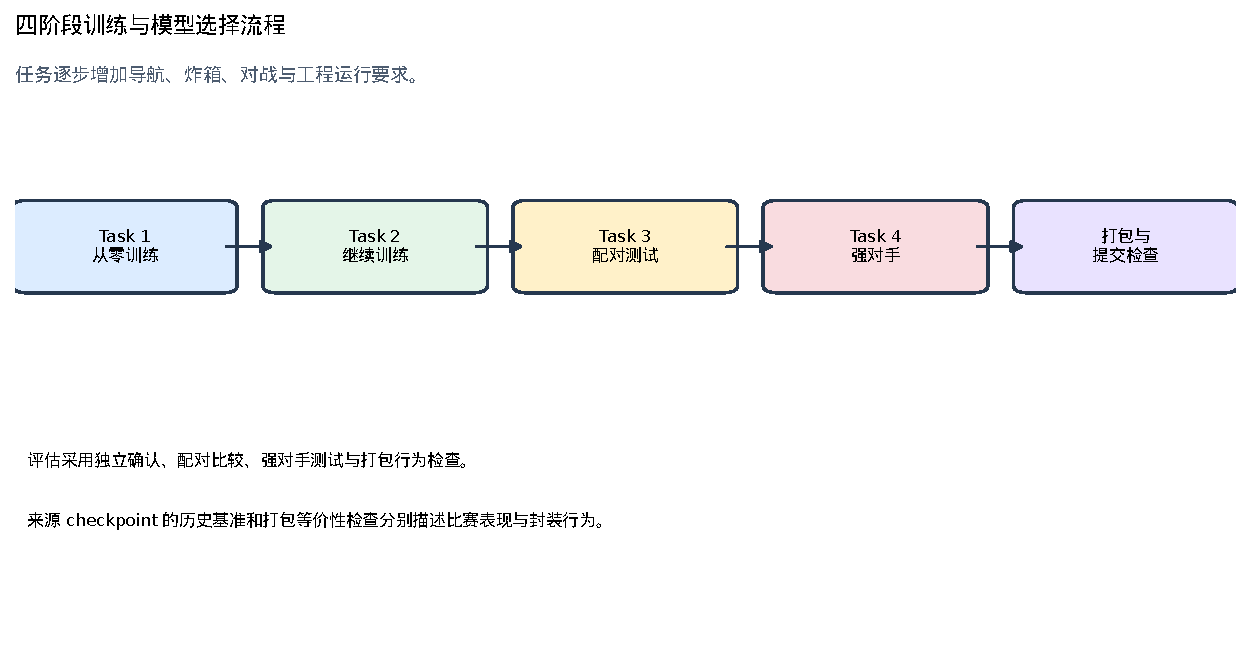
\includegraphics[width=\linewidth]{report-assets/figures/output/figure_01_curriculum_pipeline.pdf}
\caption{训练课程和模型选择流程。独立确认是在开发集选出模型后，用另一组对局检查该版本。Task 3 比较从 Task 2 模型继续训练的版本与原模型在相同世界中的逐局得分差。打包检查则在 6 局中确认重命名后的程序与来源程序产生相同的完整对局回放。Die Hardest 来源模型的 1,000 局历史成绩来自另一套测试，不能与 Task 4 专项实验直接比较。}\label{fig:curriculum}
\end{figure}

\subsection{计算资源与结果记录}
为了保留每项结果的来历，我们优先使用逐局记录和原始 CSV，并在汇总中注明来源。测试环境随机种子控制游戏世界的随机生成。同一个训练模型在多个种子上测试，表示它经历了多个不同世界，而不是进行了多次独立训练。E05 使用 GTX 1080 Ti、PyTorch 2.5.1+cu118、CUDA 11.8 和 Python 3.10 训练。最终提交包采用 NumPy 2.2.6、PyTorch 2.5.1，并以单线程 CPU 推理。

\section{方法}
\subsection{Die Hardest 的特征表示}
Die Hardest 使用团队共享的 \texttt{continuous-v2}，即把棋盘局面转成 84 个数值输入的表示。这套表示由团队成员主导开发。前 70 个数值中，60 个按六种候选动作各占 10 个，另有 10 个描述全局局面。动作顺序为 \texttt{UP}、\texttt{RIGHT}、\texttt{DOWN}、\texttt{LEFT}、\texttt{WAIT}、\texttt{BOMB}。每个动作的 10 个数值分别描述动作是否合法、执行后第 1、2、3 步所在格是否有预测爆炸危险、最早遇险时刻、预测时限内最多还能安全移动几步、最后一层安全可达格的比例，以及移动后到金币、可站在旁边放弹炸到的箱子和对手的距离变化。合法性检查棋盘边界、目标格是否可走，以及是否被炸弹或其他智能体占据。危险依据未来 $H=7$ 步的炸弹图判断。炸弹按倒计时标出爆炸格，石墙挡住爆炸。移动动作按当前棋盘上的炸弹计算，放弹动作则把一枚假设炸弹加入后再计算。最早遇险时间按 $(t-1)/H$ 缩放到 $[0,1]$，七步内都没有遇险时取 1。计算安全移动步数时，程序先固定第一步动作，再逐步展开后续可走位置，并排除危险格和被占据格。能安全到达的最远步数除以 $H$，就是安全移动时长。最后一层安全位置数除以棋盘格总数，得到安全可达区域比例。这些数值为价值网络提供了动作可执行性、风险和目标进展等信息，网络据此学习评价各候选动作。

我们用广度优先搜索（BFS）计算到三个目标的最少步数。它从智能体所在格逐层检查相邻格，因此在每步移动代价相同的棋盘上能找出最短路线。金币目标是当前可见金币，箱子目标是箱子旁边能站立且可以放弹的位置，追踪对手时则以对手所在格作为终点。石墙、箱子、炸弹和其他智能体会挡住路线。对合法动作，特征记录移动前后到目标的步数差，再除以棋盘格总数减一并裁剪到 $[-1,1]$。正数表示更接近目标。前后都无法到达时记为 0。从能到达变为无法到达时记为 $-1$，反向变化记为 1。非法动作的距离变化也记为 0。全局目标可达标记直接取自当前位置的搜索结果。放弹后的存活和可达区域也用逐步展开的搜索计算，但先假设智能体在当前位置放下一枚炸弹。只有当前允许放弹时，代码才统计爆炸范围内的箱子和对手数量，计算时石墙会挡住爆炸。不能放弹时，两项都记为 0。爆炸范围内的箱子数除以炸弹沿上下左右四个方向各自最多能覆盖的格子数之和，当前设置下，每个方向最多覆盖 3 格，共 12 格。遇墙或棋盘边界时，实际覆盖范围会缩短。这个比例表示此次爆炸覆盖到的箱子数占理论上限的多少。对手数量和存活对手数除以最多可能存活的对手数。回合进度则缩放到 $[0,1]$。这 10 个全局数值依次表示目标可达性、当前能否放弹、假设此刻放弹后的存活状态及安全可达区域比例、爆炸范围内的箱子数和对手数、存活对手数，以及当前对局进度。目标可达性分别针对金币、箱子相邻可站立格和对手。它们补充候选动作特征没有单独表达的全局目标、放弹机会和对局进展。

前 70 个数只描述当前棋盘和候选动作的后果，没有记录智能体刚才做过什么。于是，即使当前棋盘相似，模型也看不到智能体刚才是朝哪个方向移动、上一步在追哪枚金币。我们增加近期行为记录，让输入能提示动作是否会回到刚离开的格子，以及金币目标是否改变。

新增的 14 个数也分两组。前 7 个表示上一动作。六个动作各占一个位置，执行过的动作对应位置为 1，其余为 0。如果这是第一次决策，则第七个位置表示尚无上一动作，取值为 1。后 7 个数中，第一个表示本次选中的可达金币是否与上次决策选中同一格。如果两次选中同一格且都有目标，记为 1，否则记为 0。若多个金币到当前位置的最短步数相同，程序先选横坐标 $x$ 较小的。如果横坐标相同，再选纵坐标 $y$ 较小的。例如，同距时 $(2,4)$ 会排在 $(3,1)$ 前。其余六个数分别对应六种候选动作：对四个方向移动，若目的格恰好是上次决策时智能体所在的格子，就记为 1，否则为 0。\texttt{WAIT} 和 \texttt{BOMB} 固定为 0。这个比较只检查候选目的格的坐标，不检查该动作是否合法，也不表示智能体实际走回了上一格。换言之，它只提示网络某个候选动作的目的格是否落在上一格，不判断连续多步是否形成循环。智能体会在每次选出动作后保存当时的位置、动作和目标金币，供下一次决策使用。这些历史字段把上一动作、金币目标和候选目的地同当前局面一起提供给网络，使网络可以据此学习近期行为与当前选择之间的关系。

\subsection{奖励设计与安全动作筛选}
游戏得分是最终目标，但只有游戏得分这类稀疏反馈，不容易让智能体知道应如何导航和安全放弹。因此，训练中我们还加入辅助奖励：收集金币、炸毁木箱、击杀对手和存活会得到正奖励。非法动作、自杀、长时间停留和无效往返会受到惩罚。势函数奖励塑形根据状态前后的势值变化，为即时奖励增加一项。连续路线的 r7 会在智能体选择无法逃生的放弹动作时立即给负奖励，而不是等到数步之后死亡再处罚。这样做是为了把延迟出现的坏结果更直接地归到触发风险的放弹动作上。

动作掩码的既有研究主要讨论政策梯度方法，即直接优化各动作被选概率的学习方法\citep{huang2022masking}。我们则把只负责否决动作的安全层放在价值学习器前，Q 网络仍依据动作价值选择。如图\ref{fig:inference}所示，每一步先根据棋盘边界、障碍物、炸弹和其他智能体的位置排除无法执行的动作。基础 Survival Mask 再检查每个候选动作之后的 $H=7$ 步：如果在这段时间里没有任何存活路线，就否决该动作。Die Hardest 使用的 v9 还会继续检查与自己放置的炸弹有关的危险：从当前决策逐步搜索到这枚炸弹爆炸、火焰消失为止，并把对手之后可能放置的新炸弹也算入风险。系统只保留有逐步存活方案的候选动作。若强化检查没有动作通过，系统会将基础七步筛选留下的非放弹动作交给 Q 网络排序。如果基础筛选也没有动作通过，则交给 Q 网络排序的候选是物理上可执行的非放弹动作。两种情况下，Q 网络都依据自身估值选择动作，安全筛选不负责在这些候选动作中排名。

\begin{figure}[H]
\centering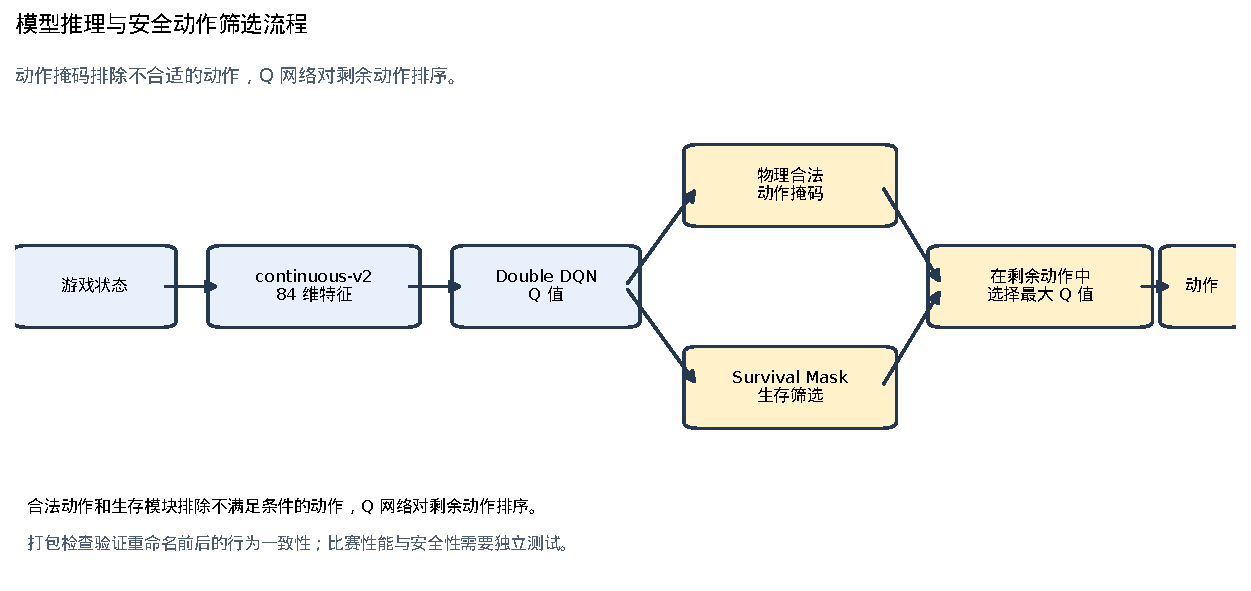
\includegraphics[width=\linewidth]{report-assets/figures/output/figure_02_inference_pipeline.pdf}
\caption{先排除撞墙或目标格被占据等无法执行的动作。基础 Survival Mask 检查未来七步内是否有存活路线，Die Hardest 的 v9 还检查自己炸弹的完整危险时段。安全层只否决未通过检查的动作，Q 网络负责给其余动作排序。}\label{fig:inference}
\end{figure}

\subsection{探索、迁移与评估方法}
训练时，$\epsilon$-greedy 探索会以概率 $\epsilon$ 随机选动作，其余时候选择当前估值最高的动作。经验回放把已发生的状态、动作和结果存起来，供后续反复抽样训练。目标网络按固定间隔从学习网络复制参数。训练检查点是某一时刻保存的模型和训练状态。恢复同一训练时，我们会同时加载模型、优化器和训练进度。迁移策略到新任务时，只加载策略参数，并重新开始该任务的探索与经验记录。如果特征、奖励或安全规则发生变化，旧经验是否仍适用需要重新核对。Task 4 的共享父模型实验让多个候选从同一份训练模型开始，减少起点不同对结果的影响。

每个任务关注的能力不同：Task 1 看金币数和收齐全部金币的对局比例。Task 2 加入炸箱、放弹后存活、自杀，以及长时间不移动等停滞现象。Task 3 关注得分、击杀和第一名比例，并在相同游戏世界中比较 Task 2 与 Task 3 模型。Task 4 还测量安全表现、等待行为、完整 \texttt{act} 调用耗时和内存。要把两个模型的结果直接比较，场景、对手、模型版本、测试世界和对局数都需要一致。

\section{训练}
\subsection{分阶段训练与模型保存点}
我们先从零训练金币导航，再在后续阶段加入木箱和炸弹。达到阶段要求后，Task 3 从 Task 2 保存的模型版本继续训练，并观察它是否保留前序能力。Task 4 则从共同的起始模型或已有候选出发，面向强对手继续训练。每次训练都记录模型配置、输入特征版本、奖励版本、安全筛选版本、训练随机种子和选中的模型版本。Task 4 的各次训练按配置和测试预算归档。

\begin{table}[H]\centering\small
\caption{各训练路线的预算记录和检查点选择方式。}\label{tab:training}
\begin{tabularx}{\linewidth}{lXXl}\toprule
路线/阶段 & 已记录预算 & 选择方式 & 关键配置\\\midrule
Double Q($\lambda$) T1 & seed 11，约 100k actions & 开发后 100 局独立确认 & $\gamma=0.95,\lambda=0.8$\\
Double Q($\lambda$) T2 & 500 局、200k actions，每 25k 检查 & 20 局开发测试 & r20，mask-v1/all\\
CNN 蒸馏 T1 & 12,825 teacher rows & 100 局开发 + 100 局 reserved & 17 通道 student\\
CNN T2 & seed 11，500 局、200k actions & 三 seed 开发后 100 局主验证 & 4-step，mask-v1/all\\
Rainbow-lite T1 & seed 11，500 局 & 20 局开发快照 & V5/r18/mask-v5\\
Continuous T3 & 三训练 seed 确认，固定 c150 & seed22 的 100-world 父子配对 & policy transfer\\
Task 4 E1--E3 & 每次约 100k actions & 100 局最终检查点 & bounded attempts\\\bottomrule
\end{tabularx}
\end{table}

\subsection{效率优化与失败修正}
我们用无图形界面的批量运行、经验回放和可恢复的训练保存点缩短迭代时间。深度网络在 GTX 1080 Ti 上训练，最终提交模型则在 CPU 上运行。测量推理耗时时，我们关闭多进程，并把特征计算、安全检查和动作排序都计入一次完整 \texttt{act} 调用。

每次遇到失败，我们都会先保存可重复检查的对局记录，再做小范围修改。Survival Mask 从 v1 到 v9 逐步更新，便于观察每项新增判断及其副作用。对局回放中的实际动作与安全计数对不上后，我们发现 Task 3 的动作选择回调和训练回调对同一决策的历史状态处理不一致，并修复了这一问题，也检查了评估代码。Task 4 中，E1 的三个训练随机种子表现不稳定，E2/E3 得分低于各自参照模型，因此这些方案按预先设定的晋级条件停止扩展。

\section{实验与结果}
\label{sec:results}
\subsection{实验设置与比较方式}
表\ref{tab:protocol}列出正文引用的主要测试。Task 1 的两个结果各来自 100 局确认测试，但测试集合不同。Task 2 中，Q($\lambda$) 的结果来自 20 局开发测试，蒸馏 CNN 使用 100 局主测试。Task 3 则让 Task 2 模型和 Task 3 模型经历相同的 100 个游戏世界。每个世界都计算一对得分，再汇总子模型减父模型的差值。Task 4 专项实验、Rainbow 测试和 Die Hardest 来源模型的历史测试使用不同对手或测试方式，因此各自报告。图\ref{fig:progression}展示各任务的能力结果，但四个面板的指标和测试不同，只能在各自面板内比较。

\begin{table}[H]\centering\small
\caption{正文采用的代表性测试，以及各结果可以如何比较。}\label{tab:protocol}
\begin{tabularx}{\linewidth}{lXrrl}\toprule
Task & 候选/测试 & $n$ & 主结果 & 结果用途\\\midrule
1 & Double Q($\lambda$)，独立确认 &100&48.95 金币&确认同一任务能力\\
1 & 蒸馏 CNN，保留确认 &100&49.84 金币&确认同一任务能力\\
2 & Q($\lambda$) r20，开发测试 &20&3.95/9 金币&选择开发模型\\
2 & 蒸馏 CNN D02，主测试 &100&2.60/9 金币&单独报告，不与 r20 排名\\
3 & 连续 DDQN 父/子配对 &100&5.91/7.14 分&在相同世界直接比较\\
4 & E1 三训练 seed 最终检查点 &各100&4.06/4.10/3.27 分&检查跨种子稳定性\\
4 & Die Hardest 来源 checkpoint 历史基准测试 &1000&4.231 分&单独报告历史表现\\\bottomrule
\end{tabularx}
\end{table}

\begin{figure}[H]
\centering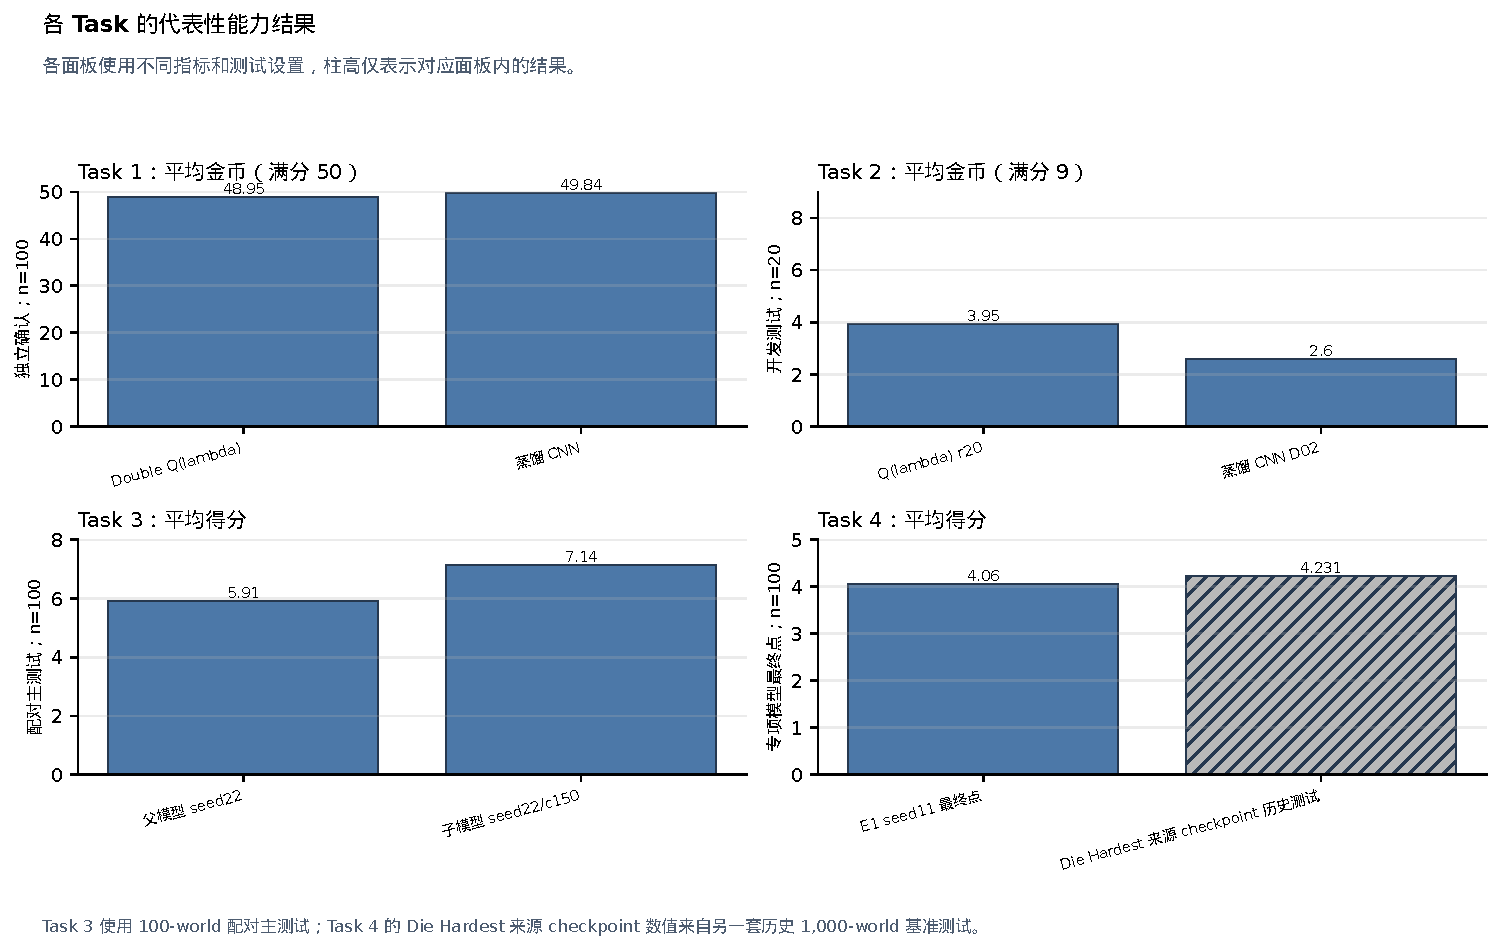
\includegraphics[width=\linewidth]{report-assets/figures/output/figure_03_capability_progression.pdf}
\caption{各任务的代表性能力结果。四个面板采用不同指标和测试设置，柱高只应在同一面板内比较。}\label{fig:progression}
\end{figure}

\subsection{Task 1：导航能力}
路径型 CNN 从 r3 到 r5 的平均金币数由 13.35 升至 41.78，全收集率也从 0\% 升至 17\%。这说明空间输入本身并不能保证稳定导航，训练设置同样重要。优化后的 Double Q($\lambda$) 在课程汇总中达到 48.95/50 个平均金币和 96\% 全收集率。原始模型日志则记录为 49.58。图表沿用课程汇总值，并保留日志值供读者核对。

蒸馏 CNN 在单独留出的测试中平均收集 49.84/50 枚金币，96\% 的对局收齐金币。一次完整 \texttt{act} 调用耗时的第 95 百分位数（P95，即 95\% 的测量值不超过此时间）为 8.39 ms，最大值为 15.55 ms。蒸馏后继续用时序差分（TD）更新网络，平均金币降至 37.21，全收集率降至 55\%，部分导航能力随在线更新而下降。Continuous DDQN 和 Rainbow-lite 选出的开发模型也都达到 50 枚金币，但它们来自不同测试设置。总体来看，多种价值学习器都学会了 Task 1，后续阶段进一步检验它们能否安全炸箱并应对对手。

\subsection{Task 2：安全炸箱与目标重选}
Q($\lambda$) r20 在 20 局开发测试中平均收集 3.95/9 枚金币、炸毁 53.45 个木箱，放弹后存活率为 100\%、自杀率为 0。30\% 的对局出现连续至少 10 步 \texttt{WAIT}，75\% 的对局出现连续至少 10 个方向交替相反的移动动作。蒸馏 CNN D02 在 100 局主测试中平均收集 2.60/9 枚金币、炸毁 44.15 个木箱，自杀率为 0。两条路线都能安全放弹，但金币收集仍低于 Task 1 水平。

连续 DDQN 的 Task 2 主测试同时保留了 Task 1 的导航能力，并取得 7.25/9 个平均金币、100.26 个木箱和 0 自杀。生存动作掩码与分阶段训练共同构成这条完整路线。Rainbow-lite 选出的开发模型在 20 局中平均收集 8.45/9 枚金币，60\% 的对局收齐金币。没有对局出现连续至少 10 步 \texttt{WAIT}，也没有对局出现连续至少 10 个方向交替相反的移动动作。该配置同时调整了输入特征、训练奖励和安全筛选，因此结果反映的是整套配置。几条路线都遇到同一个难题：炸开道路后，智能体需要根据新的可通行路线重新选择要追踪的目标。由于测试局数和模型选择方式不同，我们不把这些平均分直接排成名次。

\subsection{Task 3：弱对手与能力保持}
为了减少不同游戏世界带来的波动，我们让连续 DDQN 的 Task 2 模型和从它继续训练的 Task 3 模型在相同的 100 个世界中逐局比较。seed22/c150 指训练随机种子为 22、累计训练 150 局时选出的模型版本。每局先计算子模型得分减去父模型得分，再汇总 100 个差值，平均差为 1.23 分。95\% 配对自助法置信区间为 $[0.27,2.14]$。计算时按游戏世界重复抽取这 100 对结果，以估计平均差的不确定范围。金币和木箱结果也有所提高。击杀差的 95\% 区间包含 0，也包含平均击杀数没有变化的情况，因此不能据此断言击杀增加，详细数值见表\ref{tab:task3}。训练随机种子 11、22、33 的独立确认测试中，平均得分分别提高 1.92、1.23 和 2.56。综合来看，主验证中的增分与金币和炸箱增加同时出现，但没有证据表明击杀数也提高。

Rainbow-lite V5 c0300 在 20 局开发测试中平均得分为 7.80、平均每局击杀为 0.65、含并列第一的对局比例为 65\%。没有对局连续至少 10 步 \texttt{WAIT}。该模型来自一个训练随机种子，不能与连续 DDQN 在 100 个相同世界上的逐局差值直接比较。c250/c350 和 v11 是其他训练检查点的编号，它们的运行结果帮助我们定位局部问题。

\begin{table}[H]\centering\small
\caption{Task 3 seed22/c150 配对主验证（100 个相同世界）。}\label{tab:task3}
\begin{tabular}{lrrrr}\toprule
指标 & 父 checkpoint & 子 checkpoint & 配对差 & 95\% CI\\\midrule
得分 &5.91&7.14&1.23&[0.27,2.14]\\
金币 &3.66&4.94&1.28&[0.87,1.70]\\
木箱 &43.78&58.97&15.19&[12.17,18.16]\\
击杀 &0.45&0.44&$-0.01$&[$-0.16$,0.14]\\\bottomrule
\end{tabular}
\end{table}

\subsection{Task 4：强对手、专项实验与工程约束}
Task 4 专项实验没有形成稳定的得分提升。E1 在三个独立训练随机种子下分别得到 4.06、4.10 和 3.27 分，均记录到 0 自杀。E2 的 seed22 版本得到 2.34 分，E3 得到 2.79 分，均低于各自比较的参照模型。Frozen C 与 Frozen S 是两组设置不同的固定参数策略（测试时不再更新模型），分别得到 4.055 和 4.035 分，不能直接互相比较。整体上，这些尝试没有通过预先设定的晋级条件。

Rainbow-lite 在自己的 Task 1--3 开发测试中完成了金币导航、炸箱和弱对手任务。但在 1,000 局 Task 4 测试中，平均得分下降，连续至少 10 步 \texttt{WAIT} 的对局比例上升（数值见表\ref{tab:final}）。这显示该组合算法在早期任务中表现良好，面对强对手时仍难以持续推进目标。Rainbow-lite 和 Die Hardest 来源模型的场景、对手、测试世界及选模方式不同，因此两者的 Task 4 均分不能直接比较。

Die Hardest 来源模型此前在 1,000 局、对阵三种规则型对手的历史测试中平均得分为 4.231。含并列第一的对局比例为 50.2\%，独占第一为 37.8\%，存活率为 94.7\%。重命名并打包后，我们在 6 局中逐步比较来源程序与打包程序的动作，整局回放均一致。我们还逐条对比了 180 行观测，确认特征、动作筛选和最终动作也一致。这些检查验证改名和封装没有改变所检查的行为，不是重新测量打包后模型的比赛得分。完整 \texttt{act} 调用耗时的第 95 百分位数为 14.826 ms，最大值为 44.601 ms，峰值常驻内存（RSS）为 319.645 MB。历史比赛测试和打包检查回答的是不同问题。前者测对战表现，后者核对程序行为和运行开销。另一段失败轨迹在世界 27155 的第 77 步复现了安全筛选漏判风险的情况，表明该规则仍有边界。图\ref{fig:task4}比较 Task 4 专项模型的平均得分、完整 \texttt{act} 耗时第 95 百分位数和安全结果。

\begin{figure}[H]
\centering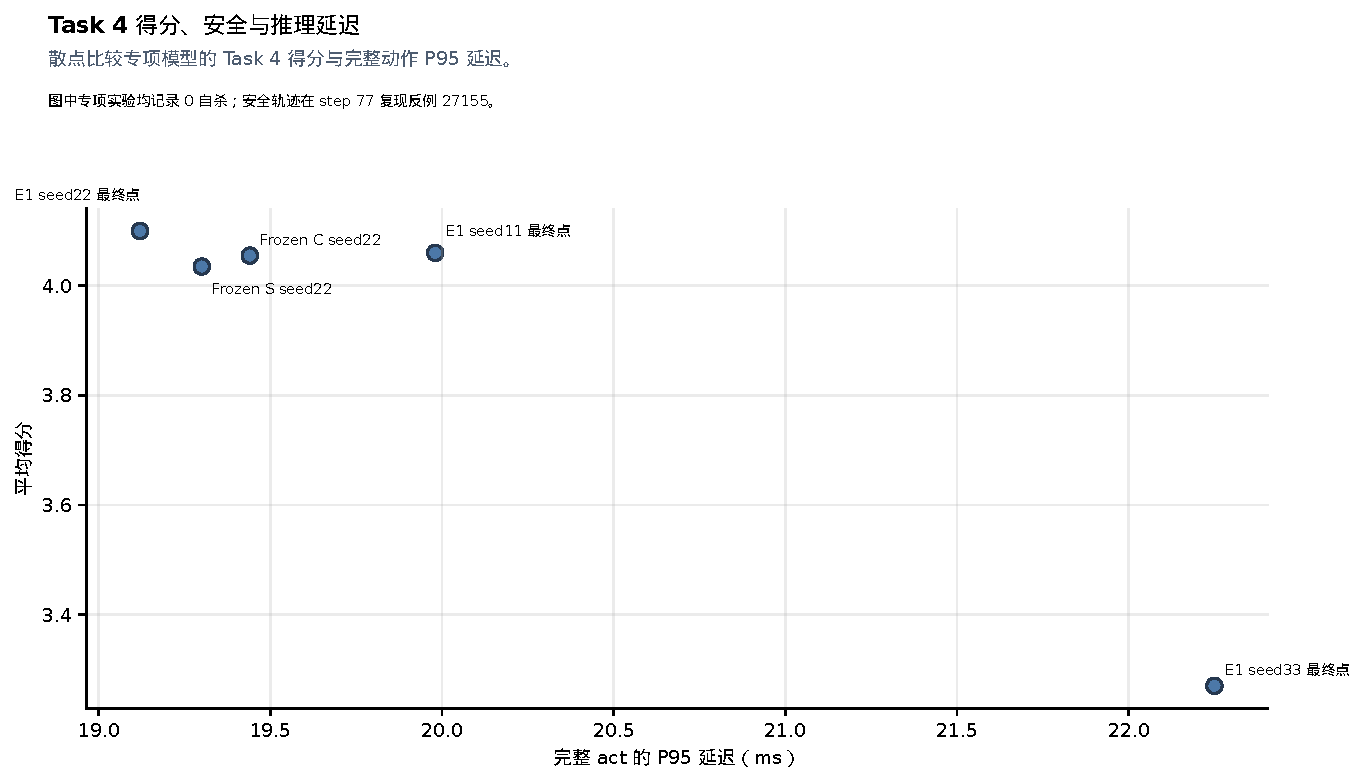
\includegraphics[width=\linewidth]{report-assets/figures/output/figure_04_task4_tradeoff.pdf}
\caption{各 Task 4 专项模型的平均得分、一次完整 \texttt{act} 调用耗时第 95 百分位数，以及各自记录的安全结果。}\label{fig:task4}
\end{figure}

\subsection{设计比较与失败分析}
把各项设计比较和失败轨迹放在一起看，可以看到三点。首先，r3 到 r5 的路径 CNN 实验同时改变了输入表示和训练设置，因此只能说明整套配置的结果不同，不能单独归因于某一项。其次，连续路线的 r7 在无法找到安全逃生路线时就对放弹动作给负奖励，试图让训练更早把之后的死亡风险归到这次放弹选择上。零自杀说明测试中没有观察到自杀，但 Task 2 中有对局连续至少 10 步等待或反向移动，Task 4 中也有长时间等待。这些现象说明智能体可能为了避险而停滞。最后，Survival Mask 只否决在七步预测内无法存活的动作，其他动作仍由 Q 网络估值排序。因此，搜索范围以外出现的风险仍可能漏过。反例 27155 展示了一次漏判。Task 3 中，回调对同一决策的历史记录处理不一致，曾使安全统计与实际动作对不上。这促使我们检查并修复评估流程。

\subsection{跨路线综合与最终选择}
表\ref{tab:final}汇总最终候选。Rainbow-lite 在早期任务表现良好，但对强对手时会长时间等待，Task 4 专项模型没有稳定提高得分。Die Hardest 来源模型有 1,000 局历史比赛结果。重命名和打包检查中，所检查对局的动作回放与来源程序一致，CPU 推理也保持稳定。结合历史成绩、运行表现和截止时间，我们选择 Die Hardest 作为提交模型。各路线的 Task 4 对手和测试条件不同，因此不能直接按均分排名。世界 27155 的失败轨迹则指出了安全筛选仍需改进的具体情形。

\begin{table}[H]\centering\small
\caption{最终候选的代表性结果与选择。}\label{tab:final}
\begin{tabularx}{\linewidth}{lXX}\toprule
候选 & 代表性结果 & 决策\\\midrule
Rainbow-lite & 早期课程表现良好，Task 4 均分 2.938，长 WAIT 比例 57.1\% & 不作为最终包\\
Task 4 specialists & E1 得分为 4.06、4.10 和 3.27，均记录 0 自杀，专项得分提升不稳定 & 停止扩张\\
Die Hardest & 来源 checkpoint 历史均分 4.231，打包行为等价，CPU 推理稳定 & 作为交付候选\\\bottomrule
\end{tabularx}
\end{table}

\section{结论}
\subsection{研究问题回答}
实验结果显示，模型复杂度本身并不能预测课程表现。表格 Double Q($\lambda$) 和蒸馏 CNN 都接近 Task 1 上限。连续 DDQN 在 Task 3 的同世界逐局比较中提高了平均得分。Rainbow-lite 虽然完成早期任务，却在强对手测试中多次长时间等待。辅助奖励和只负责筛除部分致命动作的 Survival Mask 可以用于不同价值学习器，但炸开道路后如何重新选目标、如何预见更晚才出现的危险仍是难题。选择最终模型时，我们综合考虑任务表现、前序能力保持和运行稳定性。Die Hardest 来源模型有较大规模的历史测试记录，且打包版本在核对的对局中复现了来源程序的动作，在截止时间和 CPU 约束下，我们据此选择 Die Hardest 作为最终提交模型。

\subsection{局限与未来工作}
Task 1--4 的结果要结合各自场景、对手和测试方法理解。我们的实验反复遇到两个难题：炸开道路后，智能体需要根据新出现的通路重新决定追哪枚金币或攻击哪个目标。只检查有限步数的安全筛选，也可能看不到更晚才形成的危险。世界 27155 的第 77 步复现了一次安全筛选漏判，说明实际风险可能超出当前检查范围。Die Hardest 的历史比赛结果、打包行为核对和 CPU 耗时分别来自不同检查，不能互相代替。

特征与奖励方面，84 维输入整体参与了现有实验，尚不能判断新增的 14 个历史字段是否帮助模型识别目标切换或减少折返。奖励项也在组合配置中共同训练，因此现有结果不能单独说明某一项奖励带来了什么变化。势函数奖励塑形只有在特定数学条件下才保证不改变最优策略\citep{ng1999policy}。本项目部分工程奖励不满足这些条件，所以不能据此保证最优策略不变。

如果继续这项工作，我们会让 Die Hardest、Rainbow-lite 和一个简单参照模型从同一份已训练模型开始，在相同对手、游戏世界和对局数下比较，并统一测量完整 \texttt{act} 调用耗时与内存。我们也会把世界 27155 的失败局面加入回归测试，每次修改安全筛选后都重新运行这条轨迹，检查它是否仍会漏判。未来还可固定其余输入、训练配置和评估对局，逐项移除 14 个历史特征，检验它们对目标切换和折返行为的影响。奖励项也可逐一对照，分辨各自对应的变化。安全筛选方面，则可测试如何扩大对更远处可达区域和较晚危险的评估，并探索向智能体提供追踪金币或攻击对手等全局目标。

\bibliographystyle{plainnat}
\bibliography{references}

\appendix
\section{九类模型与证据索引}
\small
\begin{longtable}{p{0.18\linewidth}p{0.25\linewidth}p{0.45\linewidth}}
\caption{项目模型族、课程用途与主要证据类型。}\label{tab:inventory}\\
\toprule 模型族 & 课程用途 & 主要证据类型\\\midrule\endfirsthead
\toprule 模型族 & 课程用途 & 主要证据类型\\\midrule\endhead
Tabular Q & Task 1--2 基线 & 导航与炸箱基线记录\\
Double Q($\lambda$) & Task 1 确认、Task 2 开发 & 导航确认及炸箱开发结果\\
CNN DDQN & 路径与空间表示实验 & 路径/空间表示与训练版本比较\\
Distilled CNN DDQN & 小网络导航与 Task 2 & 蒸馏、保留测试及微调结果\\
Continuous DDQN & Task 1--3 连续特征课程 & 连续特征课程与配对比较\\
Phase DDQN & 分阶段配置与迁移 & 分阶段配置和迁移记录\\
Rainbow-lite & Task 1--4 组合算法路线 & Task 1--4 训练与诊断记录\\
Task 4 specialists & 强对手专项尝试 & 强对手专项尝试及结果\\
Die Hardest & 来源检查点的历史基准测试与最终提交包 & 历史表现、打包等价及运行检查\\
\bottomrule
\end{longtable}
\normalsize

\section{复现与检查说明}
正文引用的机器可读结果和图表数据保存在公开代码仓库的\href{https://github.com/Jyangwakeup/MLE_final_project/tree/main/thesis/report-assets}{报告资产目录}。Task 3 的置信区间以同一游戏世界中的子模型减父模型得分差为统计单位。对同一模型重复测试不同游戏世界，不等于重新训练多个模型。不同路线的结果仍需结合各自场景、指标、对手和测试方法解读。

\end{document}
